\styledchapter[Stappen in een Machine Learning pipeline]{stappen-in-een-machine-learning-pipeline}

Een machine learning (ML) pipeline is zoals beknopt beschreven in \autoref{sec:opzetten-pipeline} een collectie van stappen dat wordt doorlopen om een model te trainen. Elke stap bevat een aantal acties dat wordt uitgevoerd. Hapke en Nelson \cite{building-machine-learning-pipelines-oreilly} benoemen een aantal voordelen bij het gebruik van een pipeline voor het trainen van modellen:

\begin{itemize}
  \item Voorkomen van bugs
  \item[] De stap waarbij de data wordt voorbereid is gebonden aan het trainen van een model. Zonder een pipeline zou het kunnen voorkomen dat een model is getraind en achteraf het proces om de data voor te bereiden is aangepast. Volgens Hapke en Nelson kan dit zonder een geautomatiseerde workflows zorgen voor bugs \cite[p.~2]{building-machine-learning-pipelines-oreilly}.
  \item Behulpzame broodkruimels
  \item[] Bij het doorlopen van de pipeline worden zaken bijgehouden zoals hyperparameters, gebruikte datasets en de modelstatistieken. Ook is te zien welk model momenteel is uitgerold. Mocht er wat fout gaan tijdens het trainen of uitrollen, is ook informatie terug te zien om het probleem te verhelpen.
  \item Standaardisatie binnen het team
  \item[] Binnen een team zal er één correcte manier zijn om een model te trainen; met de stappen in een pipeline. Dit zorgt ervoor dat er consistentie is tussen teamleden als een model wordt getraind en is het makkelijker voor nieuwe teamleden om te starten.
\end{itemize}

\section{De stappen in een pipeline}\label{sec:stappen-in-een-pipeline}
Een machine learning pipeline begint met het opnemen van data en eindigt met het ontvangen van feedback om de prestatie van het model te verbeteren. De pipeline bevat een aantal stappen zoals data voorbereiden, het model trainen en het uitrollen van het model (\autoref{fig:model-lifecycle-oreilly}). In totaal zijn er, zonder de feedback loop stap, acht stappen dat elke keer doorlopen moeten worden om een model te trainen. Om dit proces handmatig te herhalen is tijdrovend en kan gevoelig voor fouten zijn. 

\begin{figure}[hbt!]
  \centering
  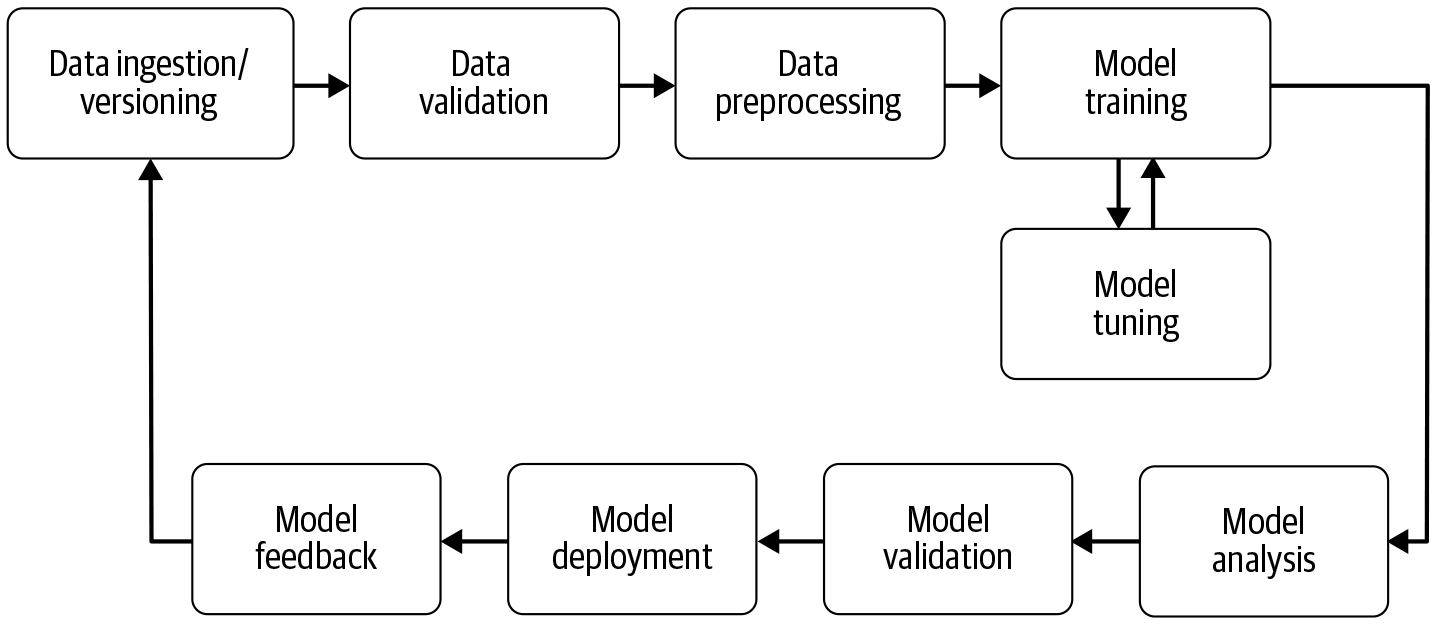
\includegraphics[width=.8\textwidth]{chapter-4/ml-pipeline-lifecycle-oreilly.png}
  \caption{Lifecycle van een model volgens Hapke en Nelson \cite[p.~4]{building-machine-learning-pipelines-oreilly}.}
  \label{fig:model-lifecycle-oreilly}
\end{figure}

Om een greep te krijgen van een machine learning pipeline zullen de stappen uit \autoref{fig:model-lifecycle-oreilly} als leidraad genomen worden. Bij elke stap in de komende subkoppen wordt code snippets gegeven. Het doel is om bij de laatste stap een werkend pipeline te maken. Een pipeline wordt doorgaans uitgevoerd in een cloud omgeving zoals Azure of Amazon Web Services (AWS). In dit hoofdstuk wordt de pipeline lokaal gemaakt en zal in \autoref{chap:cloud-computing-platformen} een pipeline in een cloud omgeving opgezet worden. 

De dataset waarmee het model wordt getraind bestaat uit 150 voorbeelden van drie iris soorten: Setosa, Virginica en Versicolor. Elk voorbeeld heeft de lengte en breedte van de kelk- en bloemblad met de bijbehorende soort iris. In \autoref{table:example-iris-dataset} is een voorbeeld van de dataset te zien. Het model zal een van de drie soorten kunnen herkennen op basis van de lengte en breedte van een gegeven kelk- en bloemblad. 

\begin{table}[hbt!]
  \footnotesize
  \centering
  \begin{tabular}{|l|l|l|l|l|}
  \hline
  \textbf{Kelkblad - lengte} & \textbf{Kelkblad - breedte} & \textbf{Bloemblad - lengte} & \textbf{Bloemblad - breedte} & \textbf{Soort} \\ \hline
  5.1 & 3.5 & 1.4 & 0.2 & Iris-setosa\\ \hline
  \end{tabular}
  \caption{Voorbeeld van de iris dataset}
  \label{table:example-iris-dataset}
\end{table}

De gekozen dataset is een bekend ML voorbeeld welk meerdere malen is opgelost. Het doel is dus om de stappen te beproeven en niet om te experimenteren met een onopgelost probleem.

\subsection{Data opname en versiebeheer}\label{subsec:data-opname-en-versiebeheer}
De eerste stap in de pipeline is het opnemen van data. Met deze data zal het model getraind, gevalideerd en getest worden. De dataset kan van een of meerdere bronnen komen, zoals lokaal, een storage bucket of van een database. Zodra de data is ingeladen, moet het verdeeld worden tussen een train, validatie en test dataset. Normaal gebeurt dit met een split ratio van 6:2:2. De train dataset is 60\% en de validatie en test dataset zijn allebei 20\% van de originele dataset \cite[p.~27-37]{building-machine-learning-pipelines-oreilly}.

Een usecase van een pipeline is dat een nieuw model getraind kan worden door een geüpdatet dataset te gebruiken. Dit wordt gedaan door de voorgaande dataset te gebruiken waarbij nieuwe data is toegevoegd. Door het gebruik van verschillende datasets is het handig om versiebeheer toe te passen. Zo is goed te zien welke dataset welk model produceert. Een versie geven aan een dataset gebeurt voordat de dataset wordt ingeladen \cite[p.~39-40]{building-machine-learning-pipelines-oreilly}. Versiebeheer voor datasets kan bijvoorbeeld met DVC \cite{dvc} of Pachyderm \cite{pachyderm}.

De iris dataset wordt in \autoref{fig:step-1} geïmporteerd door middel van code. Normaal gesproken zou, voordat deze code uitgevoerd wordt, een versie gegeven worden aan de dataset. Omdat de schaal van dit voorbeeld klein is en om de voorbeeld reproduceerbaar te houden is dit niet gedaan. De dataset wordt aangemaakt met de namen voor de kolommen op regel 5 net zoals het voorbeeld in \autoref{table:example-iris-dataset}. Vervolgens is de dataset onder de variabel naam \(dataset\) beschikbaar voor de komende stappen.

\begin{figure}[hbt!]
  \centering
  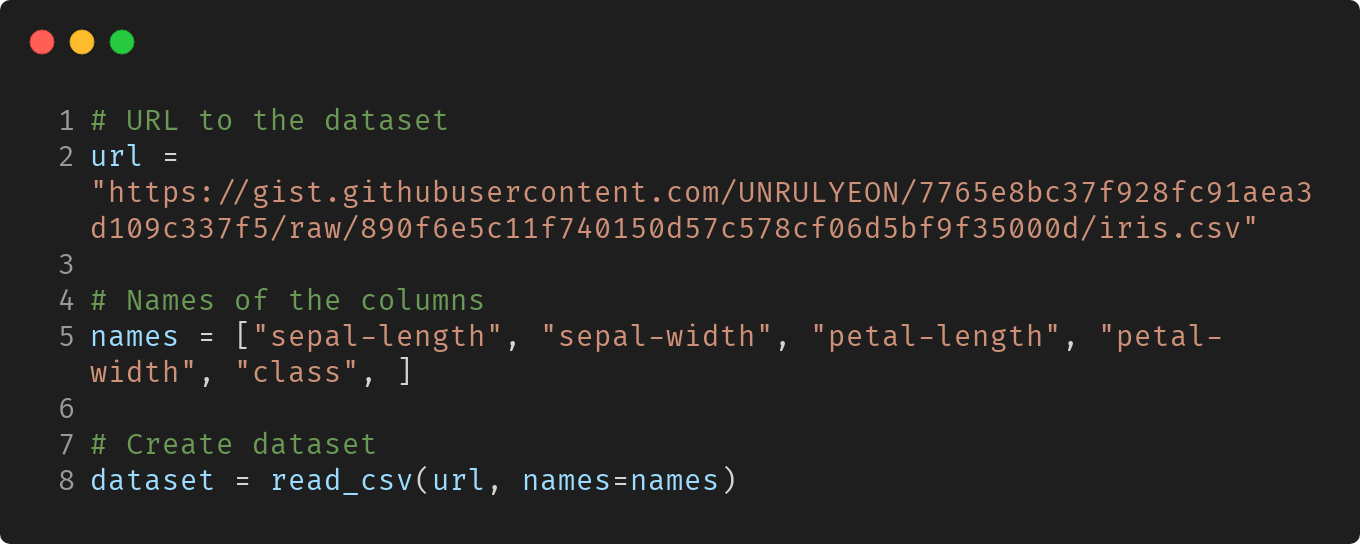
\includegraphics[width=.8\textwidth]{chapter-4/step-1.png}
  \caption{Dataset importeren}
  \label{fig:step-1}
\end{figure}

\subsection{Data validatie}\label{subsec:data-validatie}
Nu de dataset verdeeld is, een versie heeft en op een bereikbare plek is, kan de data gevalideerd worden. Deze stap is vooral belangrijk om te voorkomen dat een model wordt getraind dat niet nuttig is aangezien het trainen veel tijd in beslag kan nemen. Een bekende uitdrukking is "garbage in = garbage out". Dit betekent dat als de dataset niet goed is, het model ook niet goed zal zijn \cite[p.~43]{building-machine-learning-pipelines-oreilly}. Tijdens de validatie stap wordt gecontroleerd op het volgende:

\begin{itemize}
  \item Afwijkingen in de dataset
  \item Wijzigingen in de structuur
  \item Algemene statistieken in vergelijkingen met voorgaand datasets \cite[p.~44]{building-machine-learning-pipelines-oreilly}
\end{itemize}

Er wordt eerst statistieken gegenereerd van het huidige dataset. Om voorbeelden te geven kan een fictief dataset van woningen in Rotterdam dat te koop staat genomen worden. Uit de statistieken van dit dataset kan blijken dat er meer woningen in Rotterdam Noord zijn dan Zuid. Dit kan een onrepresentatief voorspelling geven voor woningen in Zuid. Een afwijkingen en vergelijking zou kunnen zijn dat de prijs in voorgaande datasets cijfers waren, maar in het huidige dataset karakters zijn.

\subsection{Data voorbereiden}\label{subsec:data-voorbereiden}


\subsection{Model trainen en tunen}\label{subsec:model-trainen-en-tunen}


\subsection{Model analyse}\label{subsec:model-analyse}


\subsection{Versiebeheer model (Model validation)}\label{subsec:versiebeheer-model}


\subsection{Model uitrollen}\label{subsec:model-uitrollen}


\subsection{Feedback loop}\label{subsec:feebdack-loop}


\section{Machine learning versimpelen}\label{sec:machine-learning-versimpelen}


\section{Conclusie}\label{conclusie}


\section{Advies}\label{advies}